\section{Despliegue en Kubernetes}
\label{sec:kubernetes}

Una vez validado el sistema con Docker Compose, se migró el despliegue a Kubernetes
con Minikube como clúster local. Kubernetes añade gestión declarativa del ciclo de
vida de los contenedores, sondas de preparación y la posibilidad de operar sobre
infraestructura \textit{cloud} sin modificar el código de la aplicación.

\subsection{Estructura de manifiestos}

El despliegue se define en cuatro ficheros YAML en el directorio \texttt{k8s/}:

\begin{itemize}
  \item \textbf{\texttt{studio.yaml}:} define el \texttt{Deployment} principal con
        todos los contenedores del sistema en un único pod: \texttt{voctocore},
        \texttt{telemetry}, \texttt{cam1}--\texttt{cam4}, \texttt{stream\_blanker} y
        \texttt{background\_audio}. Al compartir pod, todos los contenedores comparten
        la misma red (\texttt{localhost}), replicando el patrón del despliegue Docker.
  \item \textbf{\texttt{rabbitmq.yaml}:} despliega RabbitMQ como pod independiente
        con sus puertos AMQP (5672) y consola web (15672). Las credenciales se
        inyectan desde un \texttt{Secret} de Kubernetes para no dejarlas en claro en
        los manifiestos.
  \item \textbf{\texttt{configmap.yaml}:} centraliza los parámetros de configuración
        (resolución, puertos, rutas, host de RabbitMQ) como variables de entorno
        disponibles en todos los contenedores.
  \item \textbf{\texttt{pvc.yaml}:} define un \texttt{PersistentVolumeClaim} de 1~GiB
        para el directorio de sesiones, de modo que los registros de telemetría
        (.jsonl) persisten entre reinicios del pod.
\end{itemize}

\begin{figure}[H]
  \centering
  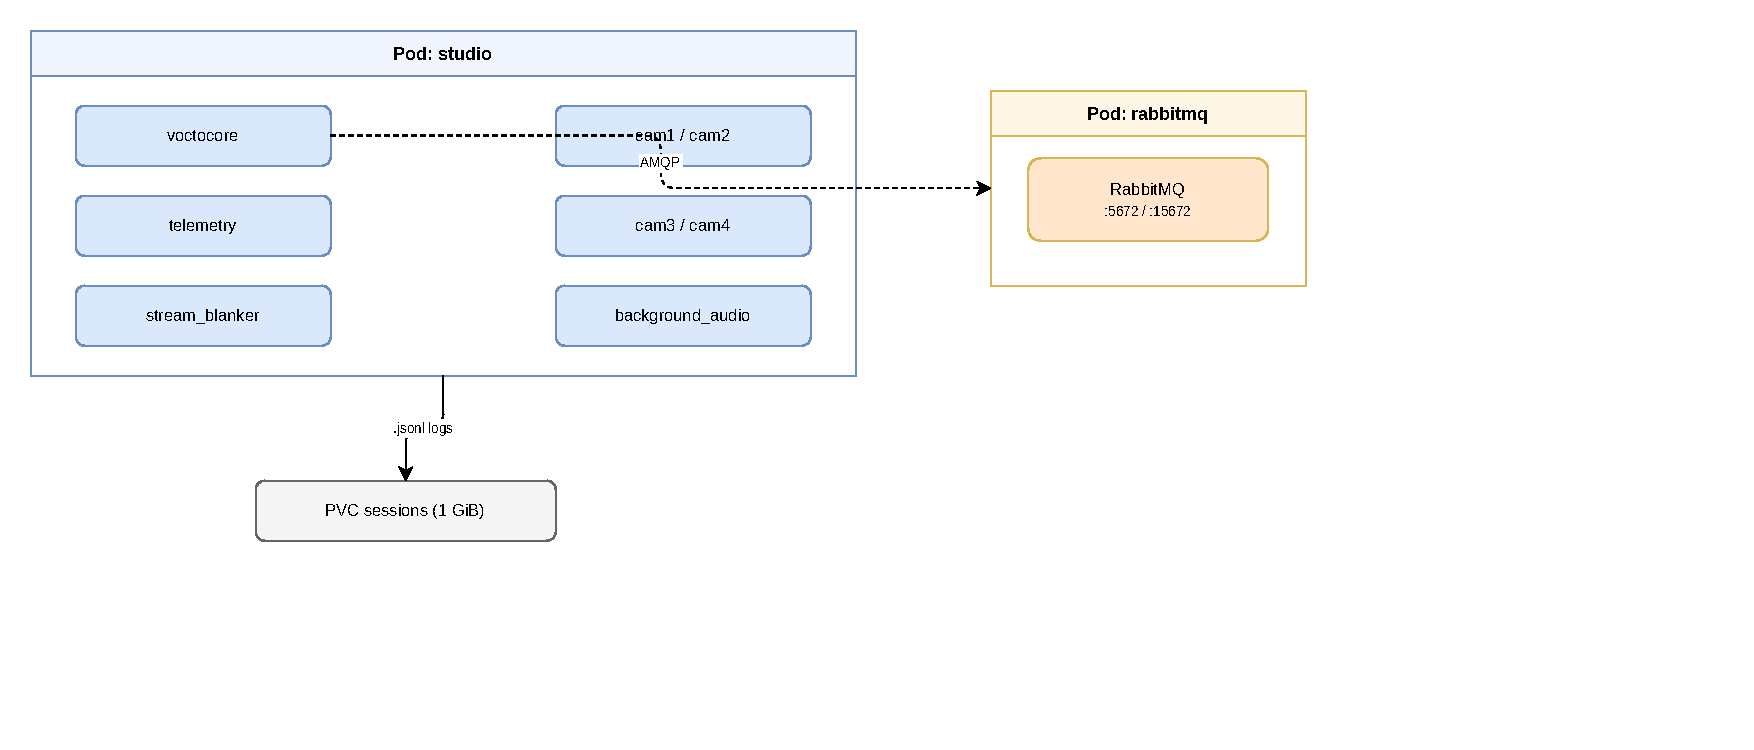
\includegraphics[width=\textwidth]{figuras/k8s_pods}
  \caption{Arquitectura de pods en el despliegue Kubernetes.}
  \label{fig:k8s_pods}
\end{figure}

\subsection{Orden de arranque y sondas de preparación}

Las dependencias entre servicios se gestionan en dos niveles:

\begin{itemize}
  \item \textbf{\texttt{initContainer} en studio:} un contenedor de inicialización
        basado en \texttt{busybox} espera a que RabbitMQ esté disponible antes de
        arrancar el pod principal (\texttt{until nc -zw1 rabbitmq 5672; do sleep 2;
        done}).
  \item \textbf{\textit{readinessProbe} de voctocore:} una sonda \texttt{tcpSocket}
        sobre el puerto 9999 determina cuándo el núcleo está listo para aceptar
        conexiones.
  \item \textbf{\textit{readinessProbe} de RabbitMQ:} ejecuta
        \texttt{rabbitmq-diagnostics ping} cada 15~segundos para confirmar que el
        broker es funcional antes de que el servicio de telemetría intente publicar
        mensajes.
\end{itemize}

\subsection{Script de lanzamiento}

El script \texttt{launch\_k8s.sh} gestiona el ciclo de vida completo: comprueba si
Minikube ya está en marcha para no relanzarlo innecesariamente, aplica los manifiestos,
espera a que todos los contenedores estén listos y establece un \texttt{kubectl
port-forward} que expone los puertos del pod en \texttt{localhost} del anfitrión.
Esto permite que voctogui se conecte al clúster igual que en cualquier otro escenario.
Al cerrar, un \texttt{trap EXIT} termina el \textit{port-forward} de forma ordenada.
